\chapter{Navigation}\label{cha:navigation}

In diesem Kapitel wird die "moving map" beschreiben, welche einen elementarer Bestandteil von \textsf{XCSoar} zur Navigation darstellt und heute selbstverständlich ist. Weiterhin werden hier die entsprechenden Elemente und Details beschrieben, welche auf der Karte eingeblendet sind, um die Navigation so schnell und einfach wie möglich zu machen.

\section{Elemente der Kartenanzeige}

\begin{maxipage}
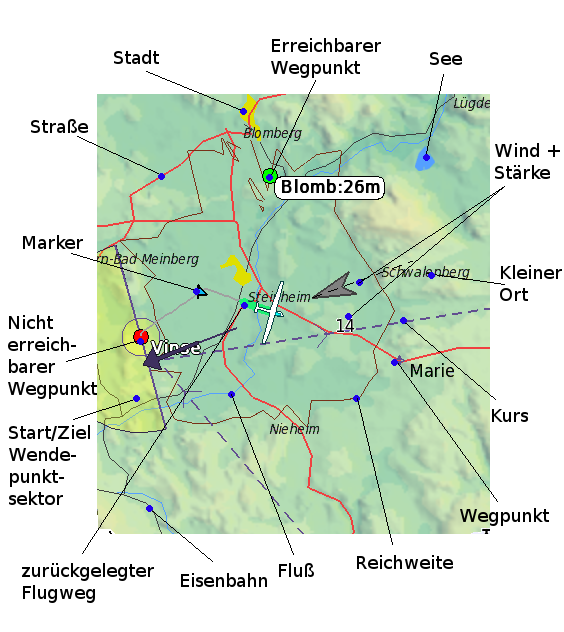
\includegraphics[angle=0,width=0.9\linewidth,keepaspectratio='true']{figures/fig-map.png}
\end{maxipage}

Die moving-map zeigt folgende Bestandteile:

\begin{enumerate}
  \item Das Segelflugzeug Symbol
  \item Die Wegpunkte
  \item Die aktive Flugaufgabe (task)
  \item Den Kurs zum gewählten Wegpunkt (bearing)
     (\footnote{Die Kurve zum nächsten Wegpunkt kann auch eine {\em Route} sein, wie es im Abschnitt~\ref{sec:route} beschrieben wird.})
    \item Die Lufträume
  \item Die Landkarte und die Topologie (Straßen, Flüsse, Seen)
  \item Markierungen (selbst erstellte "markers")
  \item Den bisher zurückgelegten Flugweg ("trail")
  \item Den Gleitbereich \footnote{Der Gleitbereich wird auch beschrieben im Abschnitt~\ref{sec:reach}.}
  \item Die aus der aktuellen Höhe erreichbaren Plätze
  \item Einen Nord-  und einen Windpfeil
\end{enumerate}

Die Karte ist in einer speziellen Projektion dargestellt, nicht in Längen- und Breitengraden. Sie kann herein- und herausgezoomt werden als auch verschoben werden. Sämtliche Navigationsberechnungen von \textsf{XCSoar} finden unter Berücksichtigung der Erdkrümmung statt.

\section{Segelflugzeugsymbol und Kartenausrichtung}\label{Segelflugzeugsymbol}\index{Segelflugzeugsymbol}\index{Kartenausrichtung}

Das Segelflugzeugsymbol zeigt die Position des Flugzeuges auf der Karte. Die Ausrichtung des Symboles gibt die ungefähre Lage des Segelflugzeuges in Bezug auf die Karte wieder(\emph{heading}).

Die Karte kann in Abhängigkeit des Flugmodus und der gewählten Einstellungen in der Konfiguration auf drei Arten dargestellt werden:

\begin{description}
\item[\emph{North-Up}] Hier wird die Karte immer in Nordrichtung (\emph{true north}) dargestellt. Das Segelflugzeugsymbol bewegt sich gemäß seinem Kurs unter Berücksichtigung des Windes.
\item[\emph{Track-Up}] Bei dieser Darstellung wird das Flugzeug immer nach oben ausgerichtet und die Karte dreht sich  mit. Hierbei wird außerdem der Nordpfeil eingeblendet, der die Richtung nach Nord angibt (\emph{true north})
\item[\emph{Target-Up}] Hierbei ist immer das Ziel am oberen Rande der Karte ausgerichtet.
\end{description}

Über die Konfigurationseinstellungen \config{orientation} können die jeweiligen Einstellungen an die Flugsituation (Kurbeln, Final etc.\  ) angepasst werden.

In den Konfigurationseinstellungen kann weiterhin eingestellt werden, ob während des Kurbelns wahlweise das Ziel oben anzuzeigen ist (\emph{Target-Up}). Dies ist evtl.\ sinnvoll, wenn während des Kurbelns kurzzeitig die Orientierung zum Ausleiten verlorengegangen ist. Nach Beendigung des Kurbelns springt die Anzeige dann wieder in \emph{North-Up} den Modus.

Wenn die Darstellung \emph{North-Up} oder \emph{Target-Up} gewählt ist, wird das Segelflugzeugsymbol in der Karte zentriert dargestellt. Normalerweise dagegen ist das Symbol ca.\ 20\% vom unteren Rand der Karte positioniert, um einen guten Überblick in Flugrichtung zu gewährleisten. Auch diese Position kann in den Konfigurationseinstellungen geändert werden.
\section{Zoom und Kartenmaßstab}\label{zoom}\label{kartenmasstab}\index{Zoom}\index{Kartenmaßstab}\index{Maßstab}
Um den Kartenmaßstab zu ändern  (für \textsf{PC}  und  \textsf{Pocket PC} ):
\begin{enumerate}
  \item Tippe auf eine leer Stelle des Displays, um die Karte zu aktivieren (keinen Wegpunkt wählen ! )
  \item Hiernach die Schaltwippe des \textsf{PDA}s hoch oder runter drücken, um herein- bzw.\ herauszuzoomen.
  \item Es können ebenfalls Gesten benutzt werden, um den Maßstab zu ändern Gesture.
      Die  \gesture{Up/Down}
     "Up'' zoomt herein,  "Down'' zoomt heraus.
     \item Als letzte Möglichkeit kann über das Menü gezoomt werden:
\begin{quote}
 \smenus{Anzeige}\blink\smenut{Zoom}{Herein} bzw. \smenus{Anzeige}\blink\smenut{Zoom}{Heraus}
\end{quote}
\end{enumerate}

Beim Altair wird der Drehknopf zum ein- und auszoomen verwendet werden.

Der Kartenmaßstab (siehe Bild links) \index{Kartenmaßstab}\index{Maßstab} ist in der linken unteren Ecke eingeblendet, weiterhin als schwarzweiß \marginpar{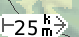
\includegraphics[angle=0,width=0.4\linewidth,keepaspectratio='true']{figures/zoom.png}}
gestreifter Balken, um je nach Maßstab die Entfernungen anzugeben(z.B.\ 0,1km, 1,0km, 10km etc.).

Die Zahl gibt hierbei die Gesamtbreite des Bildschirmes an.

Für \textsc{Compaq Aero} Benutzer: Wenn Ihr die \textsl{Compaq Aero Game Keys} aktiviert (im Q-Menü), können auch diese für das Hinein- und Herauszoomen benutzt werden.

Es besteht die Möglichkeit, zwei Zoom Einstellung zu haben: einer, wenn der Segelflieger beim Kurbeln ist, und ein weiterer welcher für den Überlandflug bzw. Endanflugmodus gültig ist.

Dies ist die "Zoom Kurbeln" Einstellung, welche unter \config{circlingzoom} eingestellt werden kann.
\halt
Als Standardmaßstab für die "Zoom Kurbel" Einstellung ist abhängig  von der Displaygröße ein Kartenmaßstab von 2,5 - 5 km voreingestellt.
Wenn während des Kurbelns hinein oder herausgesucht wird, so beeinflußt dies nicht den vorher im Grabe Ausflug eingestellten zu den Zoom-Maßstab. Sowie das kurbeln beendet wird, wird automatisch auf den vorher eingestellten Maßstab zurückgesetzt.

Die Auto-Zoom Funktion zoomt automatisch herein, wenn man sich einem Wendepunkt nähert.
Wenn Auto-Zoom aktiv ist, erscheint und links am Kartenrand ein Text "Auto-Zoom"
Es kann trotzdem weiterhin hinein und heraus gesucht werden, die Auto-Zoom Funktion wird in diesem Falle automatisch auf manuell zurückgesetzt.

\marginpar{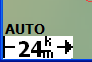
\includegraphics[angle=0,width=0.4\linewidth,keepaspectratio='true']{figures/zoomauto.png}}

Um Auto-Zoom einzuschalten, benutze folgendes Menü:
\begin{quote}
\smenus{Anzeige}\blink\smenut{Zoom}{Auto}
\end{quote}

Nachdem ein Wegpunkt sich geändert hat (automatisch, über die Wegpunkt Auswahl, oder durch manuelles Umschalten auf der Karte) wird Auto-Zoom den Maßstab automatisch so wählen, daß der nächste Wegpunkt sichtbar ist. Während des Kurbelns, wenn ein Bart entdeckt wurde, wird die Karte zentriert bezüglich des Bartes dargestellt, sodaß das Flugzeugsymbol dennoch sichtbar bleibt.

\section{Verschieben der Karte - Verschiebe-Modus}\index{Karte!Verschieben}\index{Pan-Mode}

Der Verschiebe-Modus ("Pan-Mode") erlaubt es dem Benutzer die Karte auf der moving map zu verschieben. Damit ist er in der Lage einen weit größeren Bereich zu sehen als auf den Kartenausschnitt dargestellt wird. Insbesondere bei der Aufgabenplanung ist dies sinnvoll und nützlich.
\begin{enumerate}
\item Einschalten des Verschiebe-Modus wie folgt:
\begin{quote}
\smenus{Anzeige}\blink\smenut{Verschieben}{Ein}
\end{quote}
\item Die Karte kann nun mit auf den Touchscreen gedrückten Finger verschoben werden. Auf dem \textsf{PC}  erfolgt dies mit der Maus bei gedrückt gehaltener Maustaste; beim Altair werden der innere und äußere Drehknopf hierzu benutzt.
\item Der Verschiebemodus wird verlassen mit:
\begin{quote}
\smenut{Verschieben}{Aus}
\end{quote}
\end{enumerate}

Solange der verschiedene Modus aktiv ist, erscheint der Text "Pan" und links an der Karte über den Infoboxen. Außerdem erscheint ein spezielles Verschiebe-Menü (s.u.) sowie ein Fadenkreuz, welches immer in der Mitte der Karte fixiert bleibt.
\sketch{figures/pan.png}

Der Verschiebe-Modus kann ebenfalls über Gesten aufgerufen werden \gesture{P}

\section{Wegpunkte} \label{sec:waypoint-schemes}
Die Darstellung und Einfärbung von Wegpunkten erfolgt je nach Situation und Art des jeweiligen Punktes. Hauptmerkmal ist die hierbei Landbarkeit eines Wegpunktes.  Es gibt drei Sätze für die Darstellung von landbaren Wegpunkten  (Lila Punkt, Schwarz Weiß und Ampel), die unter
\begin{quote}
\smenus{Konfig.}\blink\smenus{Konfig.}\blink\smenut{System}{Einstellung}\blink\seite{4}
\end{quote}  "Landbare Symbole" eingestellt werden können.\index{Wegpunkte!Darstellung}\index{Wegpunkte!Farben}

Die Symbole sind in untenstehender Tabelle aufgelistet. \config{waypointicons}

\begin{tabular}{c|ccc|ccc|}
Symbole
&\begin{sideways}Landbares Feld\end{sideways}
&\begin{sideways}Grenzwertig\end{sideways}
&\begin{sideways}Erreichbar\end{sideways}
&\begin{sideways}Flugplatz\end{sideways}
&\begin{sideways}Grenzwertig\end{sideways}
&\begin{sideways}Erreichbar\end{sideways}\\
\hline
Lila Punkt &

\includegraphics[width=0.8cm]{icons/winpilot_landable.pdf} &

\includegraphics[width=0.8cm]{icons/winpilot_marginal.pdf} &

\includegraphics[width=0.8cm]{icons/winpilot_reachable.pdf} &
\colorbox{white}{
\includegraphics[width=0.8cm]{icons/winpilot_landable.pdf}} &

\includegraphics[width=0.8cm]{icons/winpilot_marginal.pdf} &

\includegraphics[width=0.8cm]{icons/winpilot_reachable.pdf} \\
\hline
S/W & 

\includegraphics[width=0.9cm]{icons/alt_landable_field.pdf} &

\includegraphics[width=0.9cm]{icons/alt_marginal_field.pdf} &

\includegraphics[width=0.9cm]{icons/alt_reachable_field.pdf} &
\colorbox[rgb]{0.94,0.94,0.94}{
\includegraphics[width=0.9cm]{icons/alt_landable_airport.pdf}} &

\includegraphics[width=0.9cm]{icons/alt_marginal_airport.pdf} &

\includegraphics[width=0.9cm]{icons/alt_reachable_airport.pdf} \\
\hline
Ampelfarben & 

\includegraphics[width=0.9cm]{icons/alt2_landable_field.pdf} &

\includegraphics[width=0.9cm]{icons/alt2_marginal_field.pdf} &

\includegraphics[width=0.9cm]{icons/alt_reachable_field.pdf} &
\colorbox{white}{
\includegraphics[width=0.9cm]{icons/alt2_landable_airport.pdf}} &

\includegraphics[width=0.9cm]{icons/alt2_marginal_airport.pdf} &

\includegraphics[width=0.9cm]{icons/alt_reachable_airport.pdf} \\
\hline
\end{tabular} \\

Die Wegpunkte können nach mehreren Abkürzungsregeln beschriftet werden \seite{4}), um auf der Karte nicht so viel Platz zu verschwenden. \config{labels} Weiterhin können je nach Sichtbarkeit bzw. Erreichbarkeit die Farben und/oder Formen geändert werden. \config{labelvisibility}. \textsf{XCSoar} berechnet unter Berücksichtigung des Windes permanent, welche Wegpunkte sich innerhalb des Gleitpfades befinden.

Die angenommene Ankunftshöhe {\em oberhalb der Sicherheitshöhe} der erreichbaren  Wegpunkte wird neben dem Wegpunkt  angezeigt. Diese Ankunftshöhe wird berechnet aus der entsprechenden Leistung des Segelflugzeuges und dem MacCready Wert. Hierbei kann gewählt werden, ob die Berechnung mit einem Sicherheits-MacCready Wert, oder aber streng nach der Polare erfolgt \config{reachpolar}.

\section{Aktive Aufgabe}

Die Linie der aktiven Aufgabe wird als eine grüne, gestrichelte Linie auf der Karte dargestellt.

Bei AAT-Aufgaben werden die Sektoren der Aufgabe gelb hinterlegt dargestellt.
Die Start und Zielpunkte werden als Kreise dargestellt, Linien werden nur gezeichnet, wenn es sich hierbei um Start bzw. Ziellinien handelt.
Wendepunktsektoren werden als Segmente dargestellt (auch der DAEC-Schlüssellochsektor kann dargestellt werden).

Vom Segelflugzeugsymbol wird eine dicke schwarze Linie direkt zum nächsten aktiven Wendepunkt gezeichnet. Diese Linie stellt normalerweise den direkten Weg zum nächsten Wegpunkt dar, kann aber auch eine {\em Route} darstellen, welche um zum Beispiel Berge und/oder Lufträume herum führt. Nähere Details hierzu werden im Abschnitt Route~\ref{sec:route}  beschrieben.
\begin{center}
\begin{tabular}{c c c}
{\it Start/Ziel} & {\it Sektor} & {\it Zylinder} \\
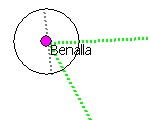
\includegraphics[angle=0,width=0.3\linewidth,keepaspectratio='true']{figures/cut-startfinish.png} &
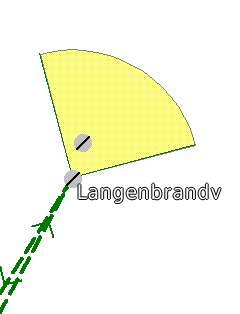
\includegraphics[angle=0,width=0.3\linewidth,keepaspectratio='true']{figures/cut-sector.png} &
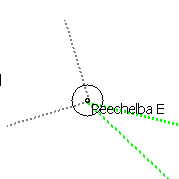
\includegraphics[angle=0,width=0.3\linewidth,keepaspectratio='true']{figures/cut-barrel.png} \\
\end{tabular}
\end{center}

\section{Gelände und Topologie}

Die folgenden topologischen Details werden auf der Karte dargestellt:
\begin{itemize}
\item Hauptstraße, dargestellt als rote Linien
\item Flüsse, dargestellt als blaue Linien
\item Große Wasserflächen (Seen), dargestellt als blaue Flächen
\item Große Städte, dargestellt als gelbe Flächen
\item Kleine Siedlungen, dargestellt als gelbe Diamanten
\end{itemize}
Großstädte und kleine Siedlungen werden in Schrägschrift beschriftet.

Das Gelände wird gemäß der Höhe eingefärbt, optional kann es schattiert werden -  entweder gemäß der Sonneneinstrahlung oder aber entsprechend des Windeinfalles (Luv oder Lee).

Unbekanntes Gelände, oder Gelände das unterhalb der Meereshöhe liegt, wird blau dargestellt.
Die Schattierung des Geländes erhöht die Erkennbarkeit der Struktur und ist derzeit so gestaltet, daß helle Flächen eines Berges die Luvseite darstellen und dunkle Flächen die Leeseite.
Die Stärke und Helligkeit der Schattierung kann konfiguriert werden \config{shading}.

Die Unterstützung der Schattierung für Sonneneinstrahlung in Abhängigkeit vom Sonnenstand ist in Arbeit\dots.
Gelände- und Topologiedarstellung kann über das Menü ein und ausgeschaltet werden:
\begin{quote}
\smenus{Anzeige}\blink\smenus{Anzeige}\blink\smenut{Gelände}{An} \\[1em]
\smenus{Anzeige}\blink\smenus{Anzeige}\blink\smenut{Topologie}{An}
\end{quote}

\begin{center}
\begin{tabular}{c c}
Topology & Terrain \\
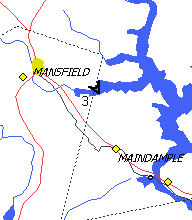
\includegraphics[angle=0,width=0.4\linewidth,keepaspectratio='true']{figures/cut-topo.png} &
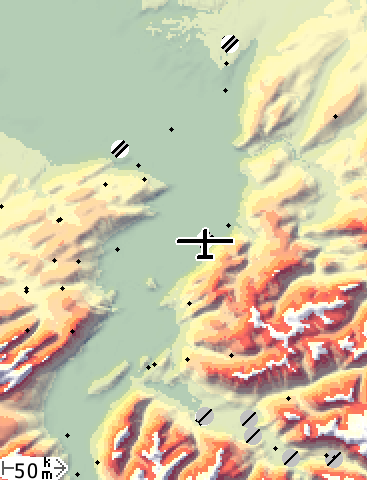
\includegraphics[angle=0,width=0.4\linewidth,keepaspectratio='true']{figures/cut-terrain.png} \\
\end{tabular}
\end{center}

Wenn keine Geländedaten zur Verfügung stehen (oder die Gelände-Anzeige ist abgeschaltet) erscheint der Hintergrund der Karte weiß. Jedes Gelände unterhalb des Meeresspiegels wird blau dargestellt!
Flüge außerhalb des in der Datenbank bekannten Geländes werden weiß dargestellt.

Um die Darstellung auf der Karte übersichtlicher zu machen, können Beschriftungen und Labels der Wegpunkte ein und ausgeschaltet werden, oder aber auf die aktive Aufgabe beschränkt werden.

\begin{quote}
%\begin{center}
\smenus{Anzeige}\blink\smenus{Anzeige}\blink\smenut{Beschriftung}{Keine}\blink\smenut{Beschriftung} {Aufgabe}\blink \dots
 %\\[0.75em] \smenut{Beschriftung}{Alle}\blink\bmenud{Beschriftungen}{Aufgabe\&}
{Landeplätze}
%\end{center}
\end{quote}

Folgende Auswahlen stehen zur Verfügung:

\jindent{\bmenud{Beschriftungen}{Aufgabe \&}{ Landeplätze}}{ Zeigt die Beschriftung der Wegpunkte  der aktiven Aufgabe und einige landbare Felder (basierend auf den Wegpunkt-Details in der geladenen Wegpunkt Datei).  Andere Wegpunkte werden angezeigt, aber nicht beschriftet. }
\jindent{\bmenut{Beschriftung}{Aufgabe}}{ Es werden nur die in der aktiven Aufgabe befindlichen Wegpunkte beschriftet. }
\jindent{\bmenut{Beschriftung}{Alle}}{ Anzeige aller Beschriftungen für alle Wegpunkte. }

Die Beschriftung und das Aussehen der Beschriftung ist über das Menü \config{labels} konfigurierbar.

\section{Flugspur (trail)}\label{sec:trail}

Optional kann die bisher geflogen Flugstrecke auf der Karte dargestellt werden. Die Farbe und die Breite dieser Spur hängt von der Höhe oder von Vario-Wert ab und kann gewählt werden. \config{snailtype}

\begin{center}
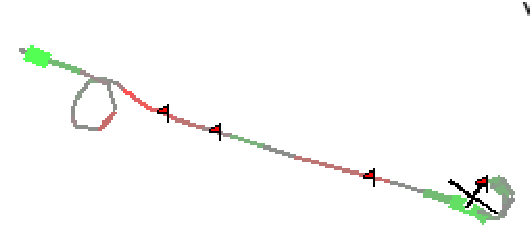
\includegraphics[angle=0,width=0.8\linewidth,keepaspectratio='true']{figures/snail.pdf}
\end{center}

Wenn das VEGA-Variometer angeschlossen ist und die Netto-Luftbewegung anzeigt, dann können die Farben und Dicken dieser Spur auch die Netto-Luftmassenbewegung darstellen.

Die Flugspur kann wie folgt ausgewählt werden: Kurz (zeigt ungefähr 10 min), Lang, (zeigt ca. eine Stunde), Voll (zeigt die gesamte bisherige Flugstrecke) und aus. Die Einstellung kann jederzeit über das Menü wie folgt vorgenommen werden:

\begin{quote}
\smenus{Anzeige}\blink\smenus{Anzeige}\blink\smenut{Flugspur}{Lang}\blink\smenut{Flugspur}{ Kurz}
\end{quote}

Alternativ kann die Einstellung auch im Menü  \config{snailtrail} als Voreinstellung werden als.
Beachtet, daß wegen der Übersichtlichkeit der Kartendarstellung beim Kurbeln die Flugspur grundsätzlich kurz ist.

Um den Windversatz beim Kurbeln darzustellen, und so das Zentrieren zu unterstützen, kann dieser Windversatz der Kartendarstellung eingeschaltet werden.

In diesem Fall wird die Flugspur relativ zum Wind aufgezeichnet und nicht mehr absolut über Grund.
Dabei hatte mit dem Wind versetzt werden, sollten die Flugspuren ebenfalls in der Kartendarstellung mit dem Wind versetzt werden. Dies, um eine bessere Anzeige zu gestatten, wie sich das Flugzeug relativ zum Bart  bewegt.

Zur Demonstration ist unten ein Beispiel beigefügt. Beachte, daß wenn die Windversatzfunktion aktiviert ist (rechtes Bild), sich das Flugzeug mehr in einem parallelversetzen Kreis  bewegt, anstelle einer gekrümmten, langgezogenen Spirale (linkes Bild).

\begin{center}
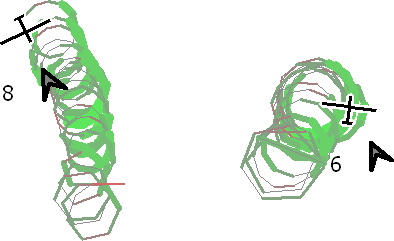
\includegraphics[angle=0,width=0.8\linewidth,keepaspectratio='true']{figures/traildrift.png}
\end{center}

Die Windversatz-Kompensation kann über die Konfiguration Einstellung ein und ausgeschaltet werden. \config{traildrift}.  Die Kompensation ist ausschließlich in Kurbelmodus aktiv; im normalen Geradeausflug wird eine Kompensation über das Wind-Menü ermöglicht:

\begin{quote}
\smenus{Konfig.\ }\blink\smenut{Wind}{Einstellung}
\end{quote}

Die Anzeige des Windversatzes zeigt sehr schön, wenn Bärte in der Höhe stark versetzt werden - zum Beispiel durch den Windscherungen.

Die Breite der Flugspur  kann optional anhand des Vario-Wertes gesetzt werden (Steigen, Saufen) \config{trailscaled}.

\section{Marker}

%
\includegraphics[angle=0,width=0.75cm,keepaspectratio='true']{icons/map_flag.pdf}

Marker werden als kleine rote Flagge auf der Karte dargestellt. Die Marker können entweder automatisch oder aber durch Knopfdruck gesetzt werden.

Ein Beispiel für die Nutzung von automatischem Setzen von Markern ist z.B. die Markierung, wann in den Kurbelmodus gewechselt wurde. Hiermit kann sehr einfach dargestellt werden, wann und wo gekurbelt wurde.

Marker werden nicht gespeichert, wenn \textsf{XCSoar} beendet wird, die Koordinaten aller Marker werden jedoch im File \verb|xcsoar-marks.txt| gespeichert.

Um Marker über das Menü zu setzen:
\begin{quote}
\smenus{Anzeige}\blink\smenut{Marke}{Setzen}
\end{quote}

Marker per Geste setzen: \gesture{Left}

\section{Anzeige des Gleitbereiches}\label{sec:reach}

Der aktuelle Gleitbereich kann wahlweise in der Karte auf zwei Weisen dargestellt werden:
entweder als schwarz-weiß gestrichelte Linie, oder aber als schattierter Bereich.

Der Gleitbereich schließt alle erreichbaren Gelände ein und markiert, entsprechende der Höhe des Geländes auch Bereich, welche evtl. umflogen werden müssen.  Dies kann sehr nützlich sein, wenn in niedrigen Höhen nach Steigen gesucht wird, oder man sich in bergigem Gelände aufhält.

Die Berechnung der Reichweite kann in zwei Detailstufen \config{turningreach} wie folgt konfiguriert werden:

\begin{description}
\item[Aus] Wenn ausgeschaltet, wird die Reichweite nicht berechnet.
\halt
\begin{center}
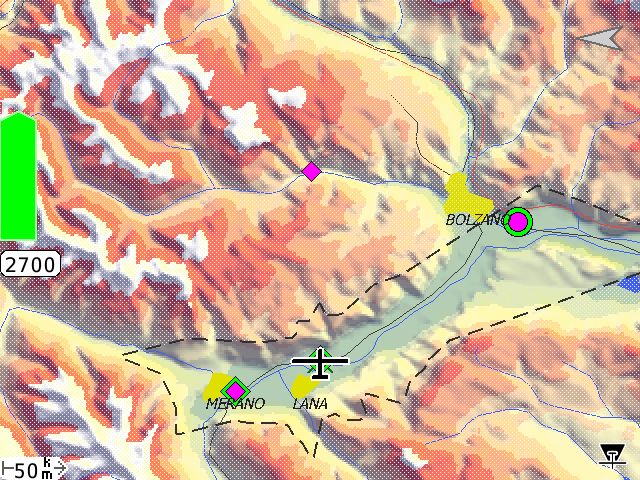
\includegraphics[angle=0,width=0.8\linewidth,keepaspectratio='true']{figures/reach1.png}
\end{center}
\item[Direkt] Wenn eingeschaltet, erfolgt die Berechnung der Reichweite geradeaus vom Flugzeug zum Ziel führenden Pfad. Es werden weder Lufträume noch sonstige Hindernisse in die Kalkulation einbezogen.
 \item[mit Umweg] Wenn dies eingeschaltet ist, wird die Reichweite unter Berücksichtigung von Hindernissen und Umwegen berechnet (Gelände und/oder Lufträume, s.o.)
\begin{center}
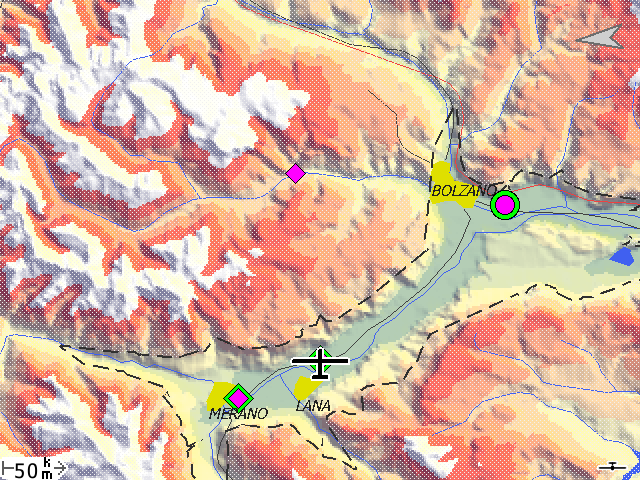
\includegraphics[angle=0,width=0.8\linewidth,keepaspectratio='true']{figures/reach2.png}
\end{center}
\end{description}

Das Display kann alternativ auch so eingestellt werden, daß das  \emph{nicht} erreichbare Gelände  verwischt / schattiert dargestellt wird.  \config{gliderange}

Der Endanflugsweg wird permanent auf evtl.\ Kollisionen mit einer Geländeerhebung geprüft - sollte sich eine Kollisionsgefahr ergeben, so wird der vorausgesagte Kollisionspunkt\index{Geländekollision} mit dem Gelände als rotes Kreuz auf der Karte dargestellt.

Wenn "Reichweite" aktiviert ist, dann wird dies automatisch wird bei Abbruch einer Aufgabe benutzt, um landbare Plätze (in allen Richtungen) auf der Karte darzustellen.

\warning Beachte, daß bei aktiven Aufgaben die "Reichweite" Funktion \textsl{in den InfoBoxen} nicht aktiv ist, hier wird die Funktion nicht verwendet!

Lediglich bei der Darstellung auf der Karte ist diese aktiv. Weiterhin wird sie verwendet für die Kalkulation der Ankunftshöhe der landbaren Wegpunkten, im Alternativen - Fenster, und im "Aufgaben-Abbruch-modus"

Die Leistungsdaten des Segelflugzeuges und die MacCready Einstellung, die für diese Berechnung verwendet werden, können eingestellt werden.  \config{reachpolar}:
\begin{description}
\item[Aufgabe] Es wird der MC benutzt, welcher in der Aufgabe gesetzt ist.
\item[Sicherheits  MC] Hier wird ein voreingestellter, i.d.R. niedriger MC Wert gewählt, den der Pilot vorher festsetzt. Normalerweise etwas schlechter als das beste Gleiten
\end{description}

\section{Status Dialog}\label{sec:aircr-stat-dial}

\begin{quote}
\smenus{Info}\blink\smenus{Info}\blink\smenus{Status}.
\end{quote}

Der Status Dialog hat fünf Unterfenster (flight, system, task rules) und dient vor allem zur Beobachtung von Zeiten, Koordinaten, Regeln etc.\

\begin{center}
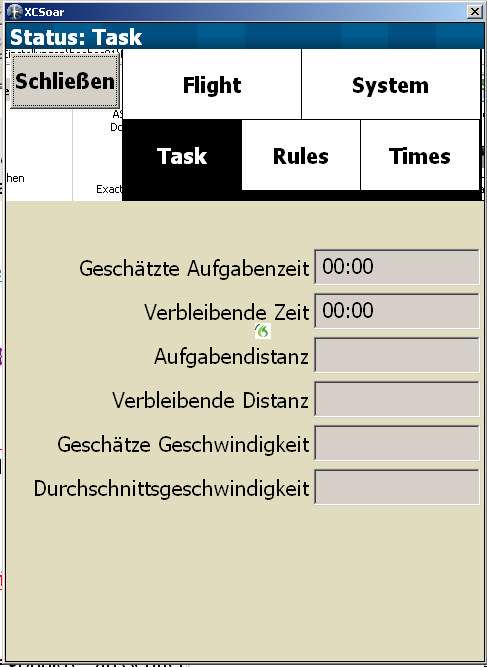
\includegraphics[angle=0,width=0.5\linewidth,keepaspectratio='true']{figures/status-task.png}
\end{center}

Die Funktion: "Flight" zeigt ein Fenster in dem der nächstgelegene Wegpunkt mit folgenden Details beschrieben wird. Koordinaten, Höhe, Entfernung, Bearing.
Sinnvoll, wenn Du Deinem Mitflieger deine Position relativ zum Dir nächstgelegenen Punkt durchgeben mußt.

Derzeit werden als "nächste Wegpunkte" ausschließlich Punkte aus der Wegpunkt-Datenbank genommen, in zukünftigen Versionen ist geplant, evtl.\  auch Dörfer und Städte aufzunehmen.

\section{Routen}\label{sec:route}

\textsf{XCSoar} kann Flugwege planen, die um Lufträume und z.B.\ Gebirge herumführen, sowohl in horizontaler als auch in vertikaler Richtung. Solch ein flugweg wird hier als Route beschrieben.

Die Höhe des Zieles ist hierbei die Ankunftshöhe des Zieles, kann aber auch größer sein, falls die Wegführung durch die in der Aufgabe deklarierten Wegpunkte dies erfordern.
Die Routen-Funktion ist in folgenden Flugmodi verfügbar:
Goto Mode, deklarierte (aktive) Aufgaben und Abort modus.

\begin{center}
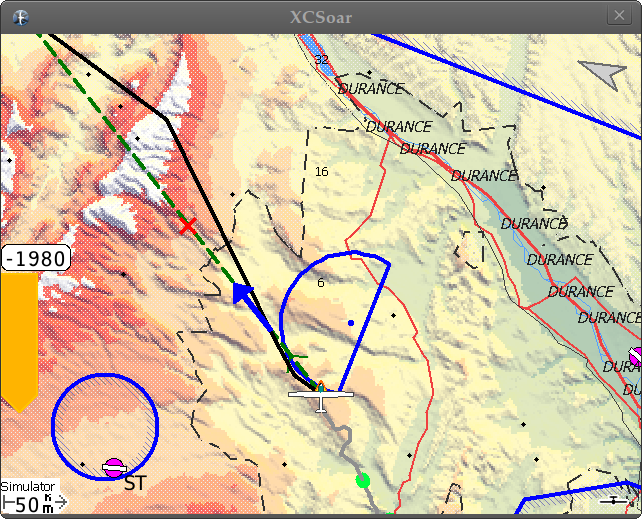
\includegraphics[angle=0,width=1.0\linewidth,keepaspectratio='true']{figures/route3.png}
\end{center}

Bei der Routenberechnung wird die Strecke unter Berücksichtgung der Flugzeugpolaren zeitoptimiert berechnet. Standardmäßig ist die Routenfunktion ausgeschaltet. Sie kann aktiviert werden unter  \config{routemode} Berücksichtigung von Lufträumen, Gelände, Wolkenuntergrenze.

Erreichbar unter:
\begin{quote}
\smenus{Konfig.}\blink\smenus{Konfig.}\blink\smenut{System}{Einstellung}\blink\seite{10}
\end{quote}

Geländekollisionen in vertikaler Richtung werden verhindert durch Einstellung der Gelände-Sicherheitshöhe. \config{safetyterrain} Hierbei ist keine zusätzliche Höhe als Puffer vorgesehen.

Es kann sein, daß manche Routen in einem  zu hohen Eintreffen des Flugzeuges an der Zielposition enden. Dies kann zum Beispiel geschehen, wenn der Zielpunkt exakt hinter einem relativ hohen Berg liegt. Zur Vermeidung von horizontalem Einfliegen in einen Luftraum wird mit ein Sicherheitsabstand von 250 m ohne weitere vertikaler Reserven benutzt.
Richtig deklarierte Routen werden im Flugverlauf über oder unterhalb Lufträumen und auf jeden Fall um Lufträume herum führen.

\warning
Wenn der MacCready-Wert positiv eingestellt wird, dann ist Steigend während einer Route erlaubt
\config{routeceiling}  Die maximale Höhe des Steigens  ist auf  500 m unterhalb der Wolkenuntergrenze limitiert, kann jedoch in der Konfiguration abgeschaltet werden.
\config{routeceiling}.
Einsteigen über die maximal vorgeschriebene Höhe des Start und Zielpunktes (siehe oben) wird "bestraft" mit einem entsprechend schlechteren Steigrate als der aktuell eingestellte MacCready-Wert
actual MacCready value.
\todonum{kapier ich nicht\dots.}

Einige Einschränkungen und Limitierung bezüglich des Routenplanungssystems sind hier aufgelistet:

\begin{itemize}
\item Wenn Kurbeln notwendig (und verboten) \todonum{hä??} ist, um das Ziel zu erreichen,  wird angenommen, daß das steigen zu Beginn der Route ist. (dies hat den Hintergrund, daß bei einer Einstellung von  MacCready gleich Null kein Steigen mehr erwartet wird (Streng nach der MC-Theorie), somit der Endanflug-Rechner in die Irre geleitet werden würde) \halt
\item Strecken mit Steigen im Geradeausflug werden auf einer konstanten Höhe angenommen, gleichbedeutend mit vielen kleinen Steigen verteilt entlang der Strecke
\item Kurven und Schlenker zwischen den einzelnen Streckensegmenten mit Ablagen größer 90° sind erlaubt
\item Fehler des Rechenalgorithmus innerhalb der Route können dazu führen, daß der Anflug in einem direkten Anflug auf das Ziel zurückgeführt wird.
\end{itemize}
